\section{Töövahendid}


\textbf{Python}

Python on üldotstarbeline programmeerimiskeel, mida kasutatakse
laialdaselt andmeteaduse, masinõppe ja ruumiandmete analüüsi ülesanneteks
oma lihtsuse ja mitmekülgsuse tõttu. Käesolevs töös kasutatakse Pythonit
andmete töötlemiseks, mudelite treenimiseks ja tulemuste analüüsimiseks.



\textbf{Jupyter Notebookid}\nopagebreak[4]

Jupyter Notebookid pakuvad interaktiivset keskkonda, kus
saab koodi kirjutada, käivitada ja dokumenteerida ühes kohas. Need võimaldavad
dünaamilist andmeanalüüsi ja tulemuste visuaalset esitlust, muutes
uurimisprotsessi läbipaistvaks ja korduvaks. Käesolevas töös kasutatakse
Jupyter Notebooke peamiselt katsetuste tegemiseks ja tulemuste
visualiseerimiseks.



\textbf{Pandas}\nopagebreak[4]

Pandas on andmetöötluse teek, mis pakub paindlikke ja
efektiivseid andmestruktuure tabelipõhise andmetöötluse jaoks. See lihtsustab
andmete puhastamist, analüüsi ja manipuleerimist. Käesolevas töös
kasutatakse Pandast andmete lugemiseks, töötlemiseks ja analüüsimiseks.


\textbf{GeoPandas}\nopagebreak[4]

GeoPandas laiendab Pandase võimalusi, lisades tuge georuumilistele
andmetele. See võimaldab lugeda, analüüsida ja visualiseerida
ruumiandmeid ning teostada geomeetrilisi operatsioone nagu lõikumine ja
ühendamine.


\textbf{Rasterio}\nopagebreak[4]

Rasterio on Pythoni teek, mis keskendub rasterandmete lugemisele
ja töötlemisele tuginedes GDAL-ile. See võimaldab ruumiandmete analüüsi
ning laseb rasterfailidega töötada efektiivselt ja intuitiivselt. Käesolevas töös oli Rasterio peamiseks tööriist rasterandmete lugemiseks ja töötlemiseks, sealhulgas satelliidipiltide koostamiseks ja maskide genereerimiseks.

\textbf{QGIS}\nopagebreak[4]

QGIS on tasuta ja avatud lähtekoodiga töölaua GIS-tarkvara, mis võimaldab
kasutajatel andmeid visuaalselt analüüsida, redigeerida ja kaardistada. See
toetab mitmeid andmeformaate ja pakub laialdasi geoprotsessimise võimalusi,
olles populaarne nii akadeemilises kui ka professionaalses keskkonnas. Käesolevas
töös kasutatakse QGIS-i peamiselt andmete visualiseerimiseks ja
analüüsimiseks, et mõista ruumiandmete struktuuri ja omadusi.


\textbf{PostGIS}\nopagebreak[4]

PostGIS on PostgreSQL andmebaasi laiendus, mis lisab ruumiandmete töötlemise funktsionaalsuse. See võimaldab keerukaid ruumi operatsioone
ja on oluline tööriist suurte ruumiandmete kogude haldamisel ning
analüüsil. Käesolevas töös autor ise otseselt PostGIS-i ei kasutanud, kuid Keskkonnaagentuuri andmebaas, kust andmed saadi, on PostGIS-i baasil üles ehitatud. Seega on see oluline komponent andmete haldamisel ja töötlemisel.

\textbf{Riistvara}\nopagebreak[4]

Uurimistöö läbiviimisel kasutati ülikooli AI-labori ressursse. Labor koosneb ühest pea-sõlmest, mis haldab teisi masinaid, ning alamsõlmedest, mis teostavad töid. Autor kasutas ai-lab-07 sõlme CPU-intensiivsete ülesannete, nagu andmekogumi koostamine, piltide töötlemine ja kompressioon, ning mitte sügav närvivõrkude mudelite treenimiseks nagu \textit{Random Foresti}. Samas süvaõppe eksperimentide teostamiseks kasutati ai-lab-04 sõlme, mille GPU ja mälumaht võimaldasid keerukamate mudelite treenimist. Selline ressursside jaotus aitas töövoogu optimeerida ja tagada tööde sujuva teostuse vastavalt konkreetsetele arvutusvajadustele.
\begin{longtable}{lllll}
    \hline
    Sõlm & Protsessor & Mälu & GPU & GPU mälu                         \\ 
    \hline
    ai-lab-07 & 3960X 24-cores/48-threads & 128 GB & NVidia 2080Ti & 11 GB    \\
    ai-lab-04 & 3970X 32-cores/64-threads & 128 GB & NVidia 3090 & 24 GB      \\
    &              &                    &                              \\ \hline
    \caption{Kasutatud riistvara}
    \label{tab:hardwareused}
\end{longtable}

\section{Andmestiku loomine}
Selles peatükis käsitletakse andmestiku loomise protsessi, sealhulgas andmete kogumist, töötlemist ja maskimist. Andmestiku loomine on oluline samm igasuguste andmete analüüsimisel ja seda ka masinõppe projektide puhul. Andmete kvaliteet ja sobivus mõjutavad otseselt mudeli täpsust ja usaldusväärsust. Nagu muudes valdkondades kehtib ka informaatikas Pareto printsiip, mille kohaselt 80\% probleemidest tuleneb 20\% põhjustest. Seega on andmestiku loomine ja töötlemine äärmiselt oluline etapp, mis võib määrata kogu projekti edasise käigu.

\subsection{Raie piirkonna andmete kogumine}
Metsateatis on dokument, mille kaudu metsaomanik esitab Keskkonnaametile
kavandatavate raietööde või oluliste metsakahjustuste kohta teabe. Keskkonnaamet
kontrollib esitatud teatiste nõuetekohasust ning veendub, et kavandatav raie
vastab kehtivatele õigusaktidele. Metsateatised menetletakse ja säilitatakse
riiklikus metsaregistris. Peale edukat menetlemist võib raietöödega alustada 10 päeva peale otsust ja kuni 24 kuu jooksul. \cite{MetsateatisJaMetsaregister} Metsateatised on avalikud ja neid saab vaadata riiklikus metsaregistris.

Metsade inventeerimise ja registrisse kandmise protsess algab metsaeraldiste
täpse kaardistamisega, kasutades L‑EST97 ristkoordinaatide süsteemi, Eesti
põhikaarti, katastriüksuse plaane ning vajadusel kaugseire andmeid eraldiste
piiritlemiseks ja võimalike situatsioonielementide täpsustamiseks. Kaardistamise
tulemusena koostatakse geoinfosüsteemi metsaeraldiste kiht, kus iga eraldis on
nummerdatud ning selle pindala, arvutatuna piiripunktide koordinaatide alusel, 
esitatakse hektarites vähemalt kümnendkohani ning täpsusega 10 meetrit --- see
loob aluse usaldusväärsele pindalaarvestusele ja edaspidistele
takseerimistoimingutele. \cite{MetsaKorraldamiseJuhend}

Koostöös Keskkonnaametiga (Envir) saadi andmed metsateatistest, mis sisaldavad teavet nii metsateatise esitamise kuupäeva, metsateatise menetlemise kuupäeva, metsateatise kehtivuse alguskuupäeva kui ka metsateatise kehtivuse lõppkuupäeva kohta. Kuna riigimetsade teatised on täpsemas seisukorras, siis võeti need raieteatised selle uurimustöö aluseks. Seoses sellega et ühe lõigu peal võib olla väga väike kogus metsa, sai teatiste pärimine ümber ehitatud sedasi, et ühe metsa raie ümber kogutakse peale raie toimumist kokku ka kõik teiste raiete raadiuses asuvad piirkonnad, millel on teada kas on mets või raieala. Piirkonniti pärimine sai teostatud kasutades PostGISi liidest Postgresi andmebaasiga. Iga raie sisaldab ka endas geomeetria veergu, mis esitab polügooni kujul selle asukohta.

% TODO: eelnevas lõigus teha arusaadavamaks, mis on lõik millest räägitakse, eelnevalt juttu kuupäevadest jm teabest ja siis võib jääda segaseks. lisaks palun täpsustada: kogutakse kokku ka teised ... raadiuses asuvad piirkonnad

\begin{figure}[hb]
    \centering
    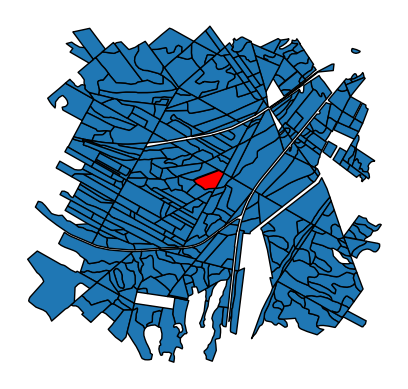
\includegraphics[width=.5\textwidth]{figures/andmestik/er_id_is10124223.png}
    \caption{Näidis ühe lageraie päringust saadud ümbrus}
    \label{fig:umbrusexample}
\end{figure}

Polügoon on geomeetriline kujund, mis määratleb kindla ala, ühendades üksteisega
punktid, et moodustada suletud piirjoon. Andmetöötluse ja ruumiandmete analüüsi
kontekstis kasutatakse polügoone, et täpselt määratleda geograafilisi alasid. \cite{WhatLocationPolygon}



\begin{figure}[H]
    \centering
    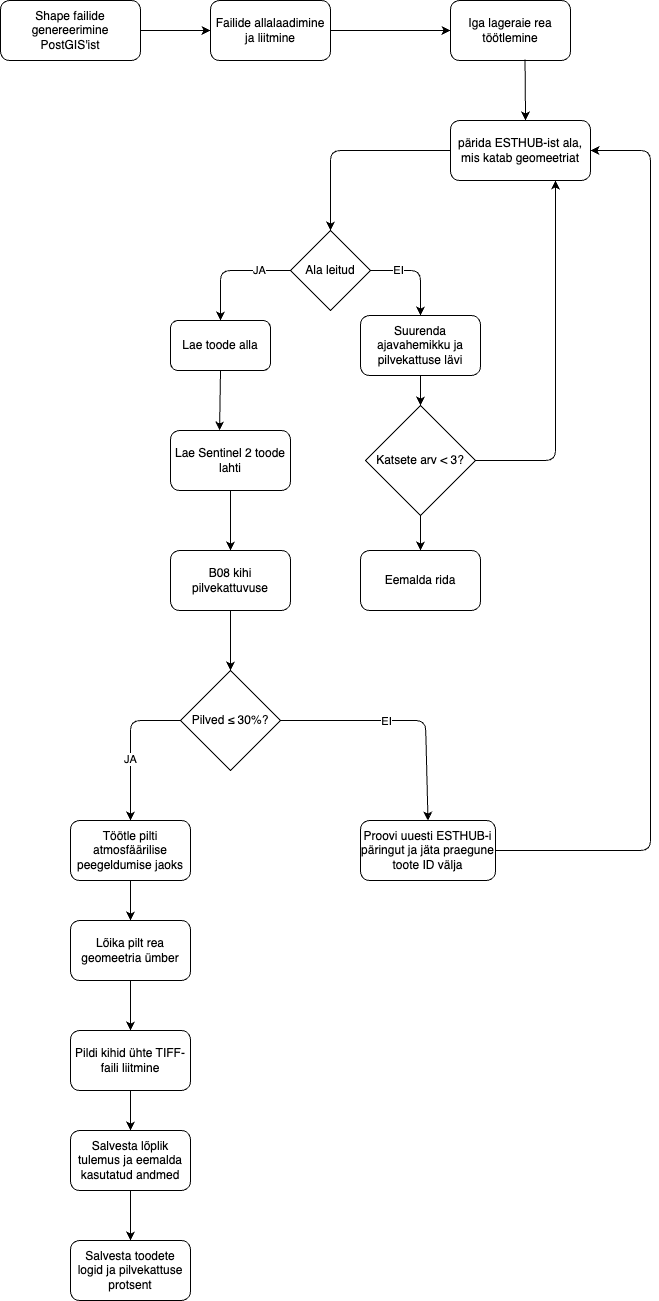
\includegraphics[width=.8\textwidth]{figures/andmestik/andmete_voog.drawio.png}
    \caption{Andmestiku loomise töövoog}
    \label{fig:terveflow}
\end{figure}


\section{Alusmudeli ülevaade}
Alustemudelid (\textit{Foundation models}) on suuremahulistel andmekogudel
ennastjuhendavalt treenitud sügavad närvivõrgud, mis toimivad üldotstarbelise
baasina mitmesuguste masinõppe ülesannete lahendamiseks. Erinevalt
traditsioonilistest mudelitest, mis on välja töötatud konkreetse ülesande jaoks
ja nõuavad eraldi treeningut, on alusmudelid eelnevalt ettevalmistatud laia
valiku ülesannete sooritamiseks --- alates loomulikust keele töötlemisest ja
tekstigeneratsioonist kuni pildiklassifitseerimise ja vastuste genereerimiseni
--- ilma täiendava märgendatud õppematerjalita. Nende mudelite
kohanemisvõime tuleneb nii suurest parameetrite hulgast kui ka enesekontrollil
põhinevast õppestrateegiast, mis võimaldab neid hõlpsasti peenhäälestada
konkreetsete rakenduste jaoks. Võimalus keskenduda mudeli peenhäälestusele ja mitte nullist treenimisele omakorda vähendab oluliselt arendusaega ja arvutiressursside vajadust.
\cite{WhatAreFoundation}

\subsection{DINO v2 võrdlus teiste mudelitega}
\input{chapters/alusmudelite_võrdlus.tex}
 \subsection{DINO v2}
\textbf{DINO v2} on Meta AI poolt loodud isejuhendatud (self-supervised) mudelite kogum,
mille eesmärk on õppida üldotstarbelisi visuaalseid omadusi ilma märgendatud
andmeteta. Mudel põhineb Vision Transformer (ViT) arhitektuuril, mille erinevad
variandid (nt ViT-S/14, ViT-B/14, ViT-L/14 ja ViT-g/14) on eelõpetatud suurel,
mitmekesise sisuga ja kureeritud pildikogumil. Mudeli struktuuri põhjaks on
õpetaja--õpilase skeem, kus õpilasmudeli parameetreid koheldakse tavalise ViT‑võrguna, aga õpetajamudeli
kaale uuendatakse õpilase kaalude eksponentsiaalse libiseva keskmise kaudu.
Treeningprotsessi stabiliseerimiseks ja tunnusruumi hajutamiseks on lisatud
Kozachenko--Leonenko (KoLeo) regulaarija, mis soodustab tunnuste ühtlast jaotust.
Õppetöö lõpus suurendatakse sisendpiltide resolutsiooni
ajutiselt 518\(\times \)518 pikslile, et parandada piksli tasemel
ülesannete, näiteks semantilise segmenteerimise ja objektituvastuse ennustuse
täpsust. Praktikas saavutab DINO v2 tänu optimeeritud
FlashAttention‑i ja PyTorch Full‑Sharded Data Parallel (FSDP) meetodile kuni
kahekordse kiiruse ning vajab kuni kolm korda vähem mälumahtu, võrreldes varasemate SSL‑mudelitega. \cite{oquabDINOv2LearningRobust2024}

\section{Seoste leidmine}
Selleks et tõestada antud magistritöö eesmärki segmenteerida lageraie ja metsa alasi suurte visioonimudelitega, klusterdatakse DinoV2 väljundid, et leida, kas need alad on eristatavad. Selleks on vajalik eksperdiga valideerida ühe lageraie piirkonna alad, et kindel olla, et need vastavad tõele satelliidipildilt.

Joonisel \ref{fig:näidisSadeliidiPilt} on näidispilt eksperimendist, mille käigus püüti välja selgitada, kas mudelid suudavad eristada lageraie ja metsa alasid satelliidipiltidelt. Antud Sentinel-2 andmebaasist saadud pilt sai valitud esiteks sellepärast, et see on hea nähtavusega, võimalikult vähe pilvine ja soojemal hooajal, kui pole lund ja puud on lehteis. Teiseks on käesolev pilt heaks aluseks, sest sellel on sattunud raie- ja metsapiirkondi kõrvuti, mis võimaldab erinevatesse klassidesse kuuluvate alade üleminekukohti analüüsida.

\begin{figure}[H]
    \centering
    \includegraphics[width=.7\textwidth]{figures/seose_leidmine/näidisSadeliidiPilt.png}
    \caption{Näidis sateliidi pilt}
    \label{fig:näidisSadeliidiPilt}
\end{figure}

Joonisel \ref{fig:raieInfoMask} on näha lageraie piirkond, mis on toodud välja tumedama roosana, ja metsa piirkond, mis on joonisel heleroosana. Tegemist on aladega, mis on teada Keskkonnaametile ja mille kohta on olemas ka metsateatis. Satelliidipilt on saadud Sentinel-2 andmebaasist ja sellel on kümnemeetrine resolutsioon. Antud pilt on saadud raie teostamise ajast kuni 40 päeva hiljem, seega mahub õigesse ajaraamistikku, et piisavalt täpselt hinnata metsade seisukorda.

\begin{figure}[H]
    \centering
    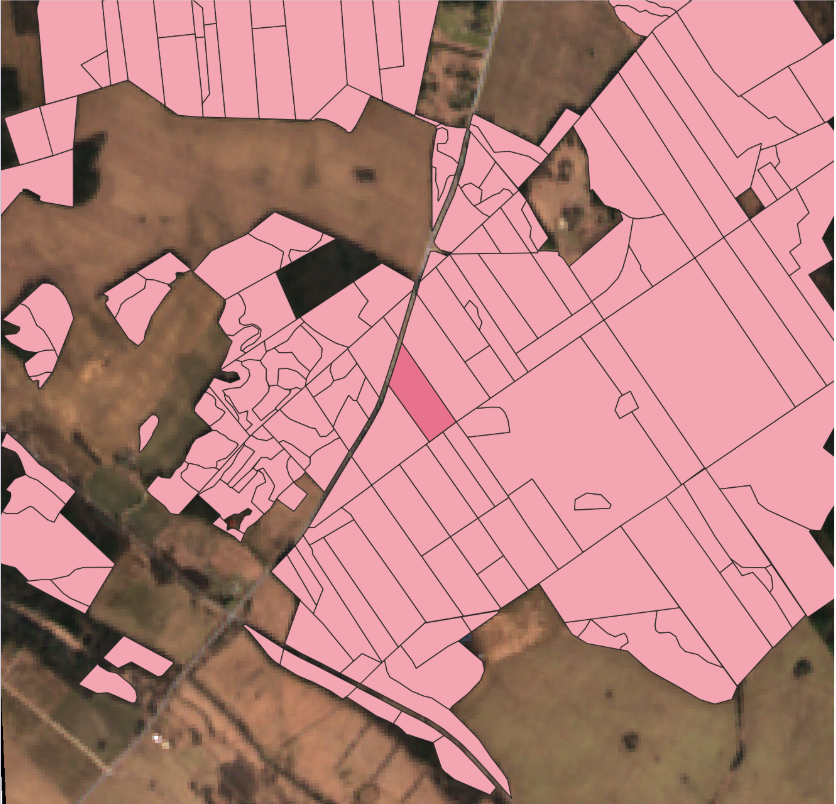
\includegraphics[width=.7\textwidth]{figures/seose_leidmine/raieInfoMask.png}
    \caption{Raie piirkonna mask sateliidi pildil}
    \label{fig:raieInfoMask}
\end{figure}

Joonisel \ref{fig:raieInfoMask_ekspert} on näha lageraie piirkond, mis on toodud välja tumepunasena ja metsa piirkond, mis on märgitud rohelisega. Ekspert on võtnud metsateatistest saadud info alade tuvastamisel aluseks, aga sellele lisaks kasutas ta ka muud teavet nagu ortofotosid ja erinevate lainepikkuste pilte, et leida täpsemad piirded metsade ja raiealade vahel. Ekspert on leidnud, et antud piirkonnas leidub alasid, mis ei vasta metsateatistes märgendatud infole. Näiteks on pildil alasid, mis teatistes on märgitud metsaks, aga silmaga vaadates kujutab hoopis raiet ja ka vastupidi. Seega on eksperdi poolt loodud mask palju täpsem ja seetõttu oli eksperdi kaasamine vajalik andmestiku loomise protsessis.

\begin{figure}[H]
    \centering
    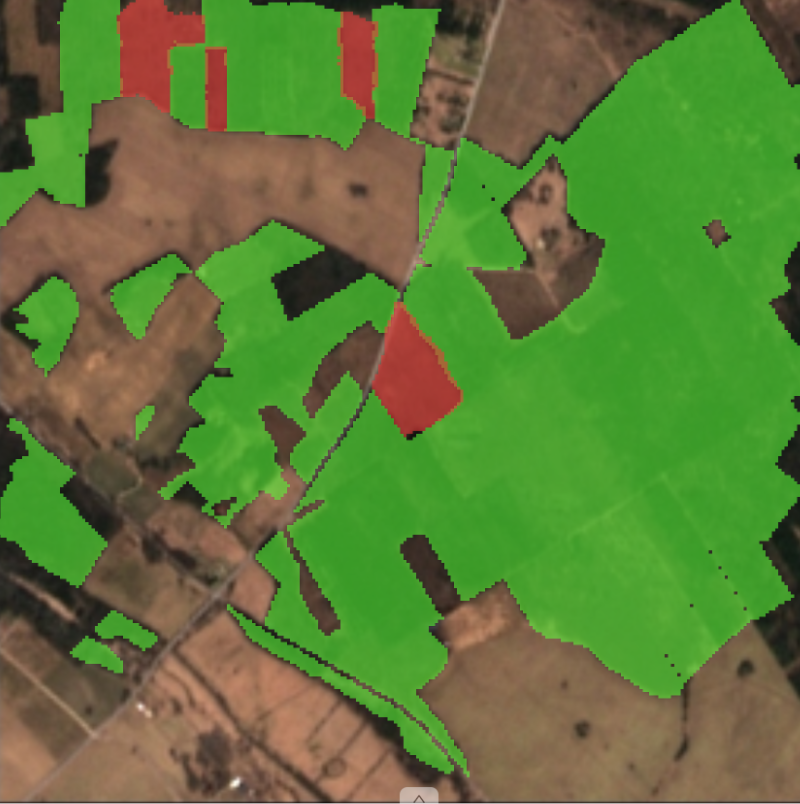
\includegraphics[width=.7\textwidth]{figures/seose_leidmine/raieInfoMask_ekspert.png}
    \caption{Raie piirkonna mask eksperdi poolt korrigeeritud}
    \label{fig:raieInfoMask_ekspert}
\end{figure}

Järgneval joonisel \ref{fig:segmenteeritudPealiskiht}, rakendati klastrianalüüsi süvaõppemudelist saadud
kõrgdimensionaalsetele tunnusevektoritele, mis esindavad sisendpildi
diskreetseid paiku. Eelkõige kasutati k-keskmise algoritmi, et grupeerida need
tunnusevektorid sarnaste semantiliste omaduste alusel. Igale pildilaigule vastav
tunnusevektor määrati ühte eelnevalt defineeritud arvu klastritesse, mille
tulemusena saadi diskreetne klastermärgis iga pildipaiga jaoks. Seejärel
visualiseeriti saadud klastermärgis pildil värvilise maskina, kus iga klaster on
esitatud unikaalse värviga, võimaldades seeläbi kvalitatiivselt hinnata mudeli
õpitud representatsioonide kohalikku sarnasust sisendpildil.

\begin{figure}[H]
    \centering
    \includegraphics[width=.7\textwidth]{figures/seose_leidmine/segmenteeritudNäidis.png}
    \caption{Segmenteeritud näidis sateliidi pildist}
    \label{fig:segmenteeritudPealiskiht}
\end{figure}

Joonisel \ref{fig:tsneDinoPatchEmbedings} on rakendatud klassipõhist klasterdamise meetodit, mille eesmärk on luua
pildimaterjalist semantiliselt sidusaid piirkondi, grupeerides pildi elemendid
eelnevalt defineeritud klassifikatsioonikategooriate alusel. Lähtudes mudeli
genereeritud klassifikatsiooniväljunditest, määratakse iga pildielement kõige
tõenäolisemasse klassi, mille alusel moodustatakse klastrid. Selle meetodi
rakendamise tulemusena saadakse segmentatsioon, kus ühte klastrisse kuuluvad
pildi osad on mudeli poolt klassifitseeritud sarnaselt. Lõppeesmärk on seeläbi
genereerida pildist arusaadavam representatsioon, mis
võimaldab interpreteerida pildi sisu semantilisel tasemel, tuues
esile objektide ja piirkondade klassipõhised seosed. Pildil on väljatoodud klass 1 mis on mets ja klass 2 mis on lageraie, lisaks sai eemaldatud tausta klass, et oleks kergem jälgida uuritavaid klasse.

\begin{figure}[H]
    \centering
    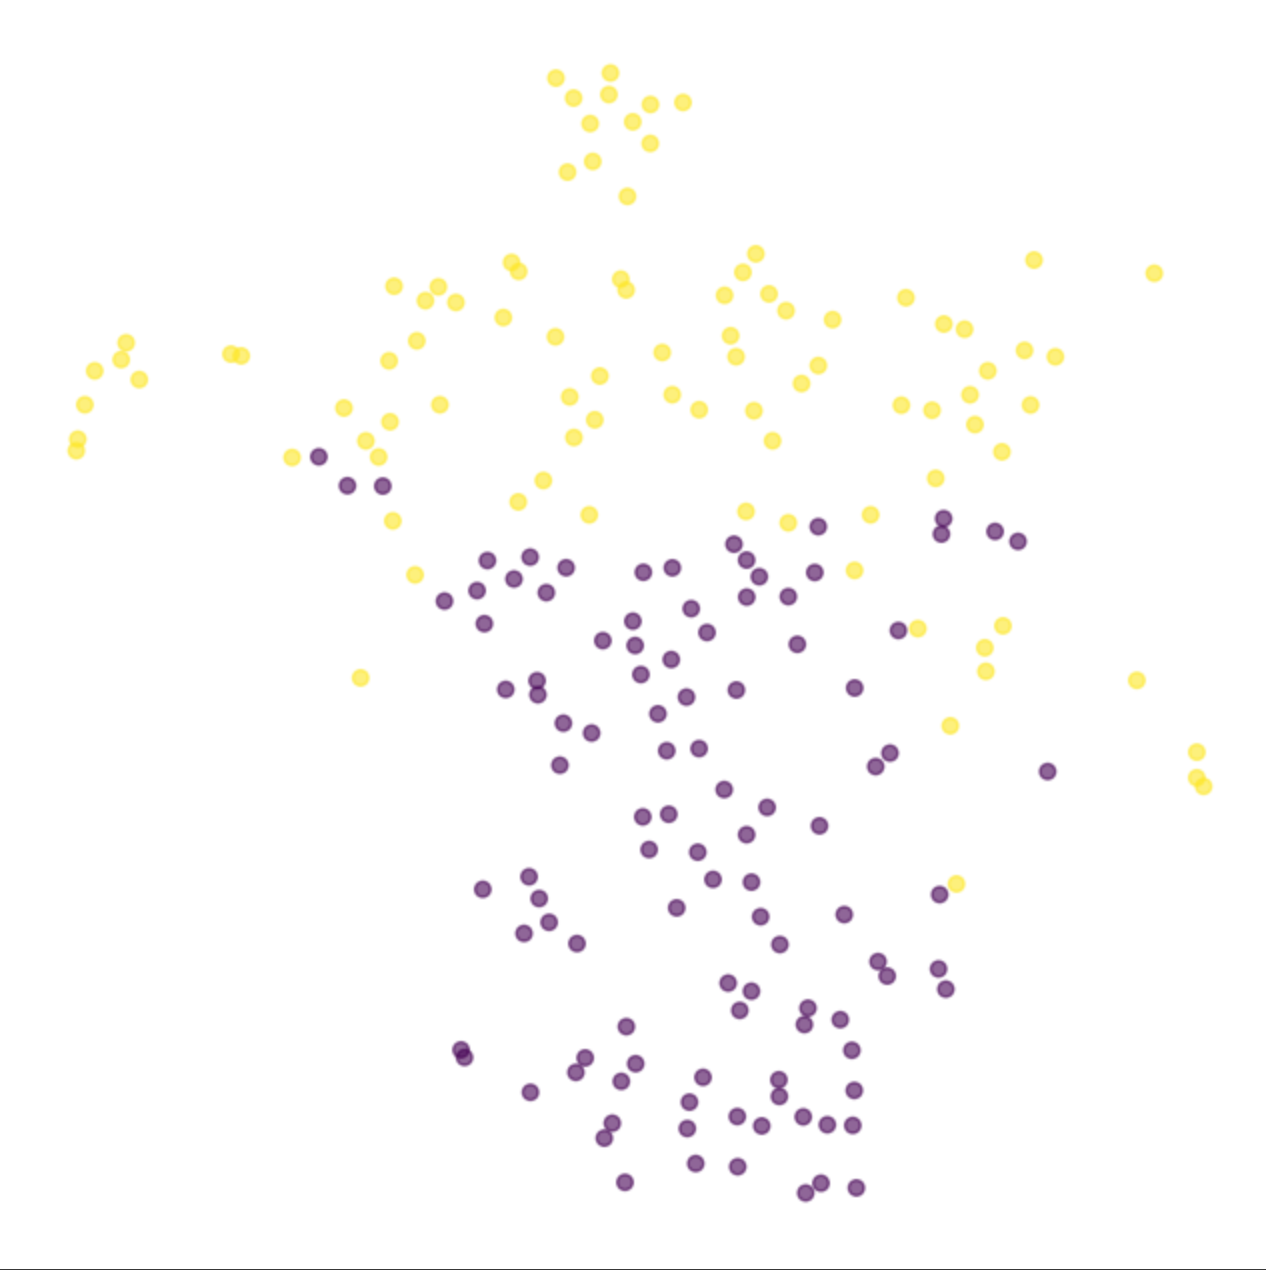
\includegraphics[width=.7\textwidth]{figures/seose_leidmine/tsneDinoPatchEmbedings.png}
    \caption{T-SNE kluster analüüs DinoV2 mudeli väljunditest}
    \caption*{klass 1 - mets, klass 2 - lageraie}
    \label{fig:tsneDinoPatchEmbedings}
\end{figure}

Siit võis näha, et lageraie ja mets on eristatavad ja annavad alust edasi uurida, millised alusmudelid suudavad paremini eristada lageraie ja metsa alasid.

\section{Treenimis protsetuurid}